\section{RouteBastion}
\label{sec:routebastion}


% \subsection{System Context} \label{subsec:system_context}

While traditional solutions like Google Cloud's or Azure's VRP APIs focus on providing a singular API interface for optimization, RouteBastion is architected to act as an intelligent broker that dynamically selects the most suitable API from multiple providers based on a variety of metrics, such as cost, performance, and input size limits. This API selection adds a layer of flexibility that is uncommon in existing systems, which generally require manual selection or are tied to a single provider. For such, we present an overview of RouteBastion architecture using the C4 model notation \cite{c4model} in Figure~\ref{fig:system}. RouteBastion interacts with two main entities: 
\begin{itemize}
  \item \textbf{External Software System}: This represents any server-side application that interacts with RouteBastion to request route optimizations or query the status of ongoing optimizations. The external system relies on RouteBastion to route these requests to the most appropriate cloud provider based on dynamic factors like cost and performance.

  \item \textbf{Cloud Provider}: These are VRP optimization API providers such as Google Cloud and Azure, which provide the computational resources and algorithms to solve the Vehicle Routing Problem. RouteBastion connects with these providers, leveraging their APIs to perform route optimizations for external software systems.
\end{itemize}

\begin{figure}
  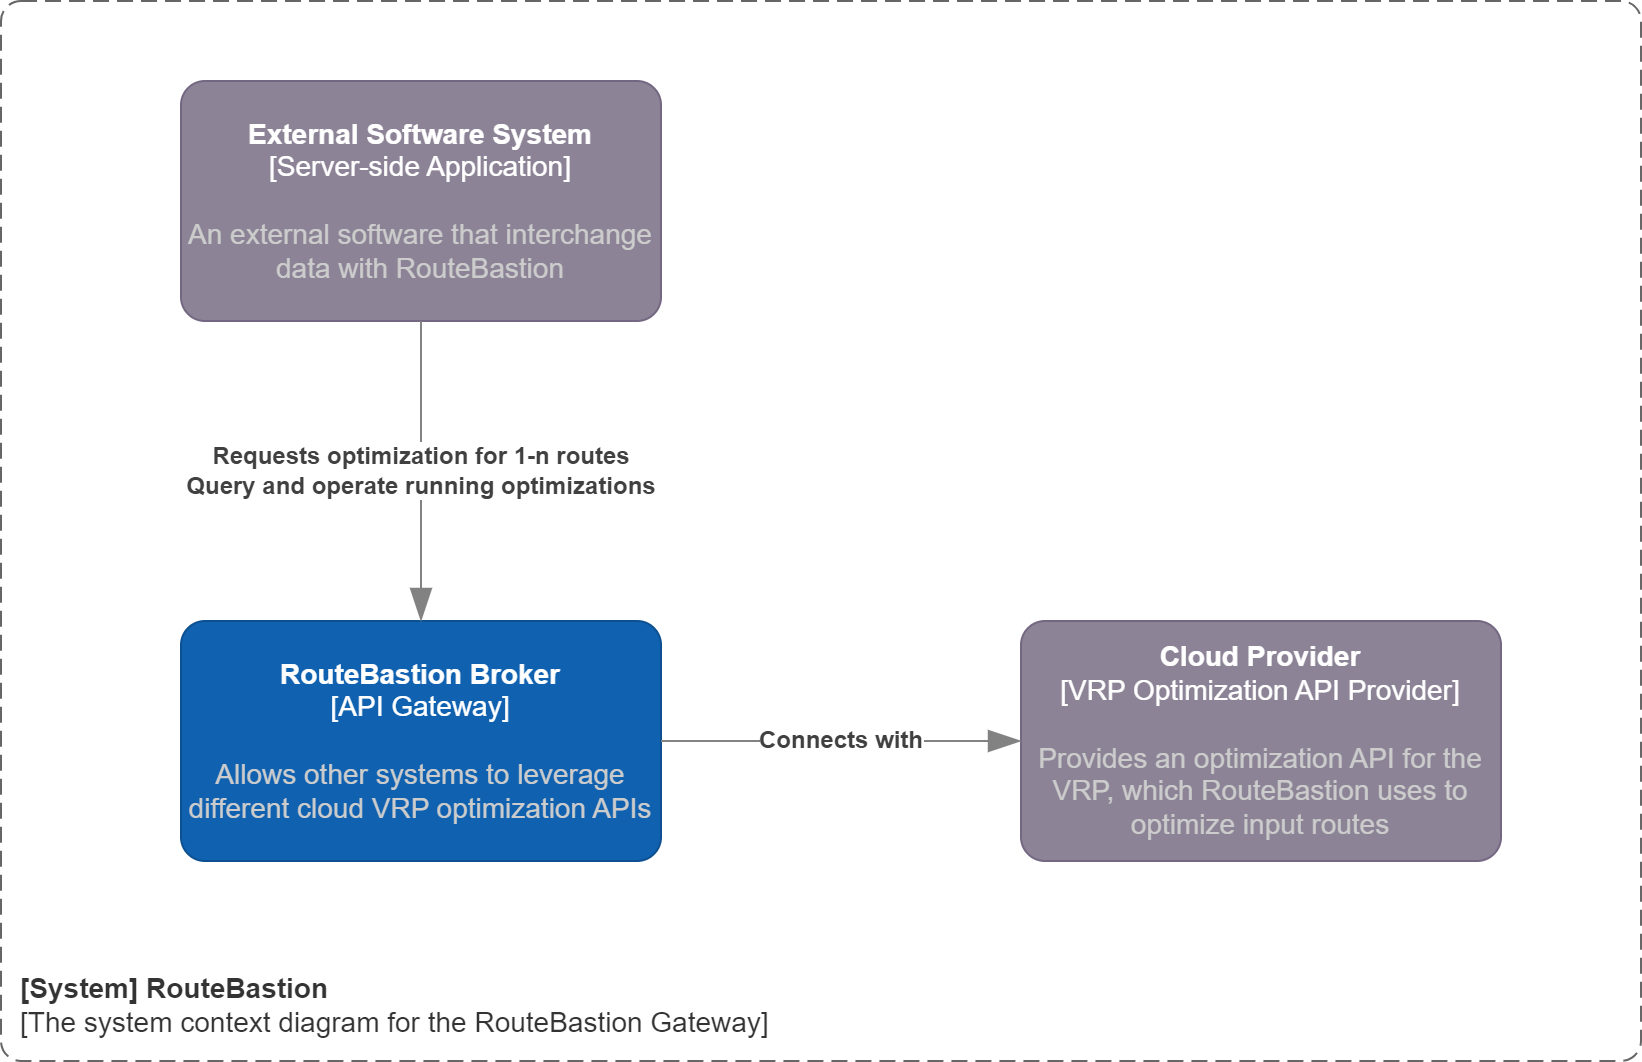
\includegraphics[width=\columnwidth]{figures/c4_diagrams/System_Bigger.png}
  \caption{System Diagram.}
  \label{fig:system}
\end{figure}

% \subsection{Container Architecture}

At the heart of this architecture is the RouteBastion Broker, which serves as the API gateway and manages the selection and routing of optimization requests to the cloud providers. The dynamic cloud provider selection algorithm poses unique challenges, as it must balance performance, cost, and other metrics without introducing significant overhead.

The container diagram, shown in Figure~\ref{fig:container}, delves deeper into the internal components of the RouteBastion Broker system, highlighting the service itself and databases that power the platform. The key components of the architecture include:

\begin{figure}
  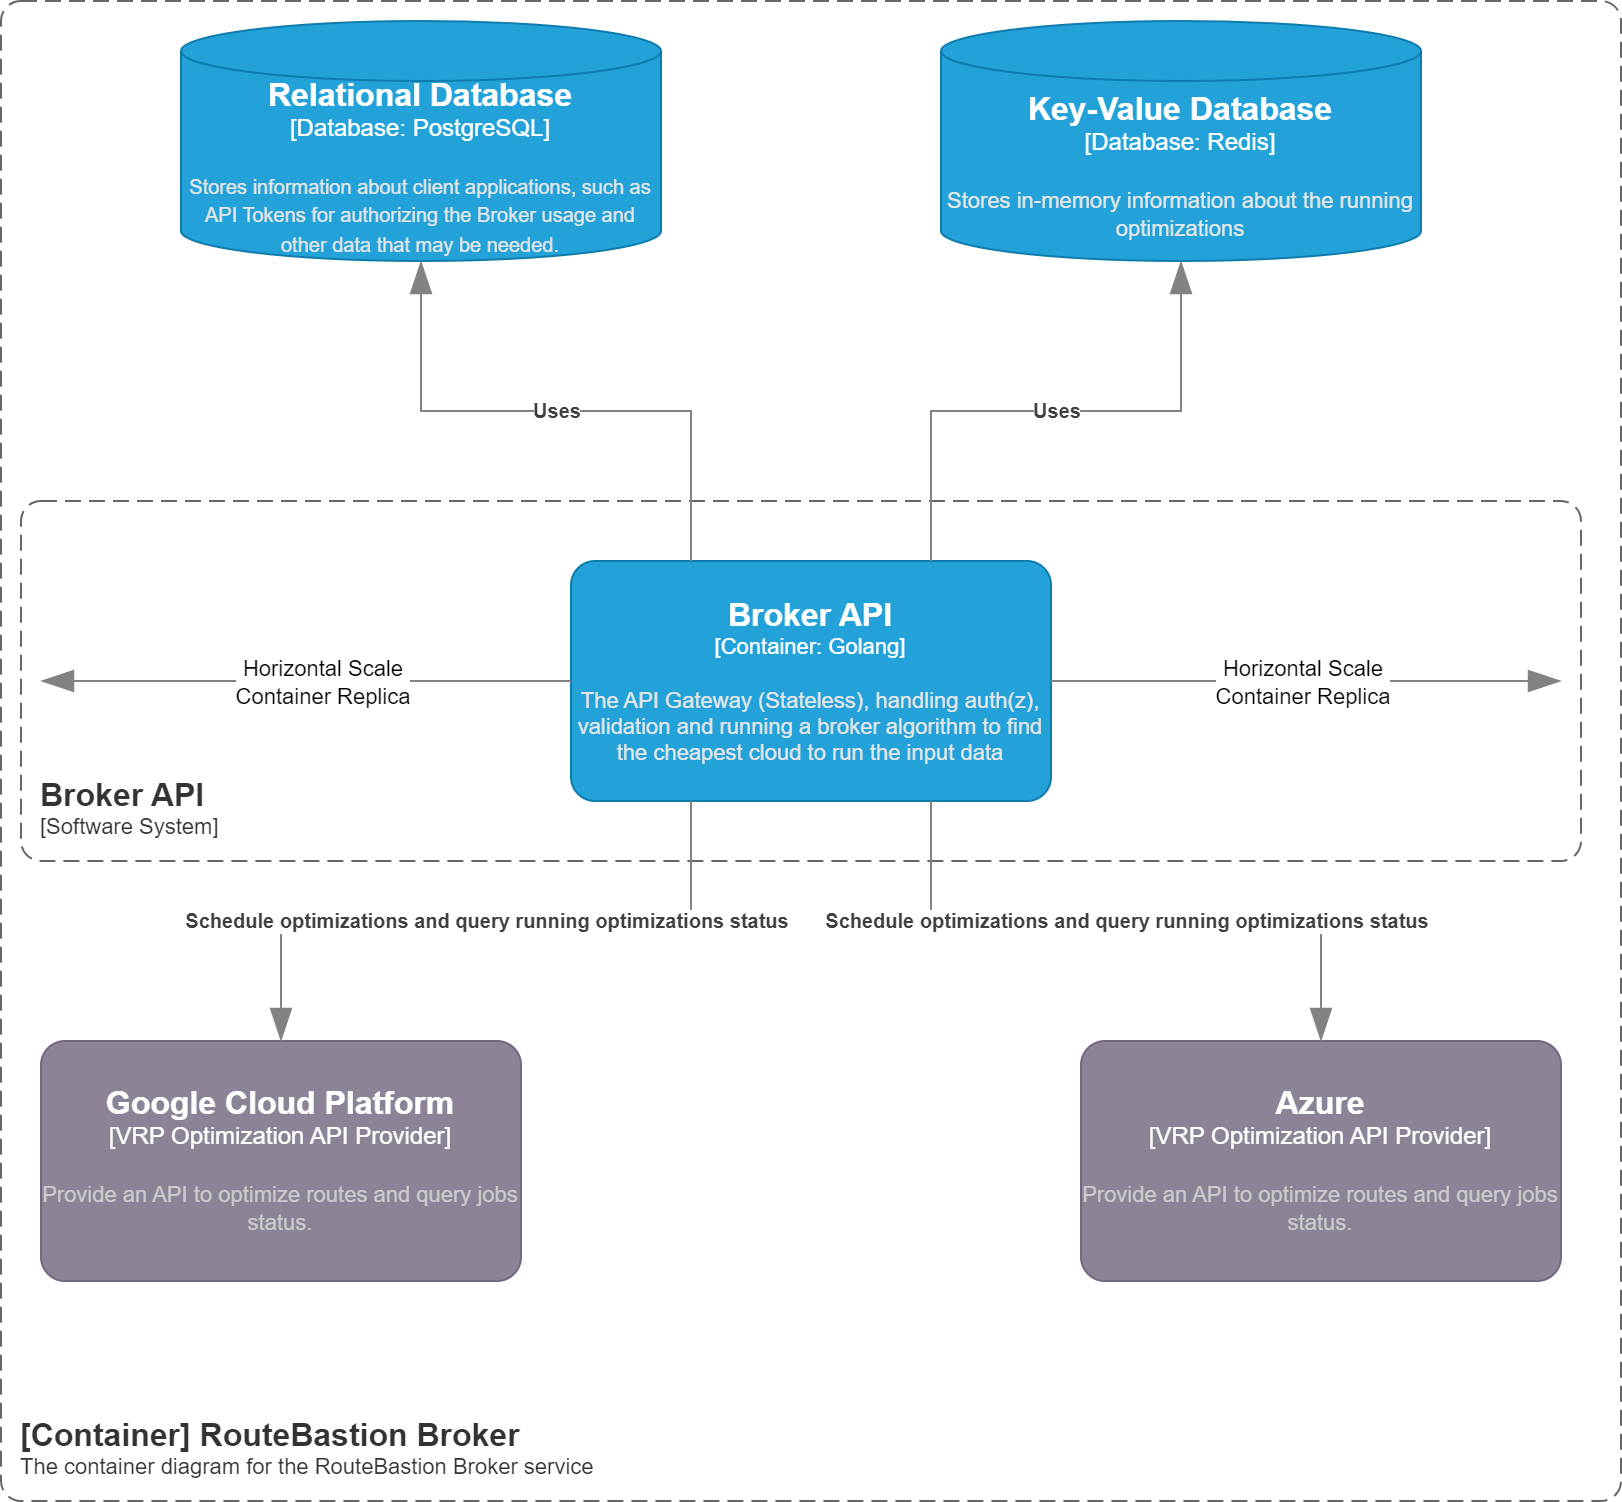
\includegraphics[width=\columnwidth]{figures/c4_diagrams/Container.png}
  \caption{Container Diagram\label{fig:container}}
\end{figure}

\begin{itemize}
  \item \textbf{Broker API}: The Broker API is the main container, which acts as a stateless API gateway, handling authentication/authorization, request validation and running a broker algorithm that dynamically selects a cloud provider. The Broker API is horizontally scalable, meaning that additional replicas can be deployed to handle increased loads, ensuring the system can process high volumes of route optimization requests simultaneously.

  \item \textbf{Relational Database}: This component (e.g., PostgreSQL)  stores persistent data, such as information about client applications (e.g., API tokens for authorization), usage statistics, and other metadata required for managing the system's operations.

  \item \textbf{Key-Value Database}: This component (e.g., Redis) is used to store in-memory data about running optimizations. It allows the system to quickly access real-time information, such as the current status of optimizations, which is essential for monitoring and querying the ongoing optimization processes.

  \item \textbf{Cloud Providers}: These are external services such as Google Cloud and Azure, which provide the actual optimization algorithms and computational power to solve the VRP. The Broker API schedules optimization jobs with these cloud providers and retrieves job statuses, allowing it to present the results back to the external software systems.
\end{itemize}

In summary, while existing systems provide powerful APIs for solving the VRP, RouteBastion differentiates itself by serving as a broker with intelligent, dynamic selection capabilities and a scalable, efficient architecture that optimizes for both performance and flexibility. This introduces new technical challenges, such as state synchronization and decision-making at scale.
